\documentclass[a4paper]{article}
%\usepackage[T1]{fontenc}
\usepackage[english]{babel}

\usepackage{amsmath}
\usepackage{amssymb,amsfonts,textcomp, graphicx}
\usepackage{graphics}

\usepackage{wrapfig}

\usepackage{parskip}

\usepackage{color}
\usepackage{array}
\usepackage{hhline}
\usepackage{subcaption}

\usepackage{textcomp}

\usepackage[hidelinks]{hyperref}

\setlength\tabcolsep{1mm}
\renewcommand\arraystretch{1.3}

\setlength\voffset{-1in}
\setlength\hoffset{-1in}
\setlength\topmargin{0.7874in}
\setlength\oddsidemargin{0.7874in}
\setlength\textheight{10.118099in}
\setlength\textwidth{6.6932993in}
\setlength\footskip{0.0cm}
\setlength\headheight{0cm}
\setlength\headsep{0cm}


\begin{document}

\newcommand\textstyleEmphasis[1]{\textit{#1}}
\renewcommand{\contentsname}{Table des mati\`eres}
\renewcommand\refname{R\'ef\'erences}

\renewcommand{\abstractname}{Pr\'eambule}
\title{\textbf{Projet Circuits Int\'egr\'es Radiofr\'equence \\ Conception d'un LNA \`a 2.45 GHz \\ en Technologie 0.35 $\mu$m AMS}}
\author{Mohamed Hage Hassan \\ Cl\'ement Cheung}
\date{12 D\'ecembre 2017}
\maketitle
\thispagestyle{empty}

\tableofcontents
\clearpage

\iffalse

\begin{figure}[!htb]
\begin{center}
  \includegraphics[scale=0.47]{Echantillonneur-bloqueur.png}
  \caption{Sch\'ema d'un \'echantilloneur-bloqueur \`a capacit\'e commut\'ee}
\end{center}
\end{figure}

\begin{figure}[!htb]
  \begin{subfigure}[t]{.5\linewidth}
      \centering
      \includegraphics[width=1.1\linewidth]{circuit-RC.png}
      \label{fig:rccircuit}
  \end{subfigure}%
  \begin{subfigure}[t]{.5\linewidth}
    \centering
    \includegraphics[width=1.1\linewidth]{sim-inital.png}
    \label{fig:rccircuit-sim}
  \end{subfigure}%
  \caption{Sch\'ema et Simulation du circuit}
  \label{fig:RC-sim}
\end{figure}

\fi

\section*{Introduction}
\addcontentsline{toc}{section}{Introduction}

L'amplificateur faible bruit constitue un \'el\'ement essentiel dans de nombreuses architectures
de recepteurs RF : il constitue normalement le premier bloc dans la cha\^ine de r\'eception et
doit se caract\'eriser par un faible ``Noise Figure'', ainsi qu'une lin\'earit\'e importante et
une tol\'erance vis-\`a-vis de la puissance des signaux parasites de fortes puissance en entr\'ee.

On \'etudie donc la topologie cascode du LNA qui est consi\'er\'ee l'une des meilleurs par rapport
au compromis entre une faible tension Vdd, stabilit\'e et le facteur de bruit NF. L'\'etude sera
men\'ee sur la bonne adaptation du montage en entr\'ee et sortie, augmentation du gain ainsi
que la r\'eduction de facteur de bruit.

\section{Conception du LNA - Partie th\'eorique}
On essaye de concevoir l'amplificateur faible bruit (figure. \ref{lna-ams})

\begin{figure}[!htb]
\begin{center}
  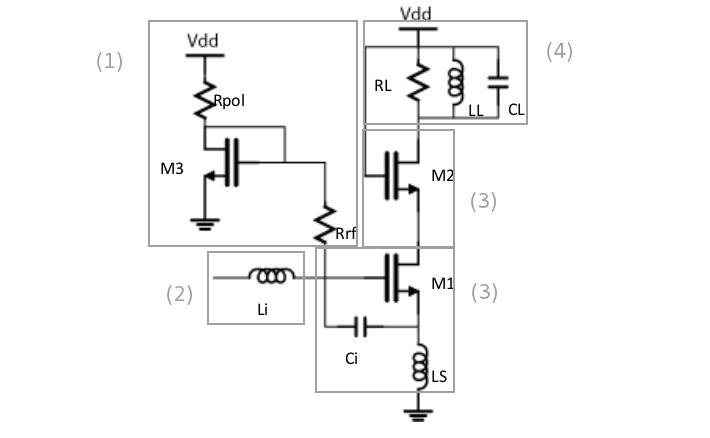
\includegraphics[scale=0.47]{lna-anotated.png}
  \caption{Sch\'ema de l'amplificateur faible bruit\cite{RFIC-tp-lna}}
  \label{lna-ams}
\end{center}
\end{figure}

Le sch\'ema comporte :
\begin{enumerate} \itemsep -3pt
  \item Circuit de polarisation du transistor $M_1$ pour avoir $I_{DS0}$ voulu
  \item Inductance de chock $L_i$ pour adapter l'imp\'edance d'entr\'ee.
  \item \'Etage cascode avec l'adaptation pour augmenter le gain du LNA ainsi de r\'eduire l'effet Miller due \`a la capacit\'e $C_{gd}$ du transistor $M_1$.
  \item Circuit r\'esonant parall\`ele RLC pour adapter l'imp\'edance en sortie.
\end{enumerate}

Le LNA doit respecter un cahier de charge bien d\'efini :
\begin{itemize} \itemsep -3pt
  \item $Gv = 20 (26 db)$, $F = 1.5 (1.76 db)$, $IIP3 = -10 dbm$
  \item $F_0 = 2.45 GHz$
  \item$\gamma = 0.82$
  \item $C_{ox} = 5 \times 10^{-3} pF/\mu m^2 $, $k_n = 80 \mu A/V^2$
  \item Courant de polarisation : $I_{DS0} = 1.5 mA$
  \item Capacit\'e en sortie $C_L = 1 pF $
  \item $Q_e = 2$
\end{itemize}


\subsection{Calcul de la charge}
On cherche $L_L$ pour r\'esoner \`a $2.45 GHz$ : Pour un circuit RLC parall\`ele,
la fr\'equence de r\'esonance est donn\'ee par :
\[
  \omega_0 = \frac{1}{\sqrt{L_L C_L}} \implies L_L = \frac{1}{(2\pi F_0)^2 C_L}
\]
Pour $F_0 = 2.45 GHz$ et $C_L = 1 pF$, on a $L_L = 4.21 nH$.

\textbf{Calcul de $g_m$:}\\
Connaissant $L_L$ et le facteur de bruit F, on cherche \`a retrouver la transductance $g_m$ :
\[
  F = 1 + \frac{\gamma}{50 gm} \frac{1}{Q^2_e}
\]
\[
  \implies gm = \frac{\gamma}{50 (F-1) Q^2_e}
\]
Ce qui nous donne $g_m = 8.2 \times 10^{-3} \Omega^{-1}$, pour $Q_e = 2$, $F = 1.5$ et $\gamma = 0.82$.

\textbf{Calcul de $R_L$:}\\
Pour $G_v = 20$, $g_m = 8.2 \times 10^{-3} \Omega^{-1}$, et $Q_e = 2$, on a :
  \[
    G_v = g_m R_L Q_e \implies R_L = \frac{G_v}{g_m Q_e} = 1.219 k\Omega
  \]

\subsection{Dimensionnement du transistor et calcul du r\'eseau d'entr\'ee}
\textbf{Capacit\'e totale $C_i$ // $C_{gs}$:}\\
Le coefficient de qualit\'e $Q_e$ pour un circuit RC s\'erie :
\[
  Q_e = \frac{||X||}{R} \phantom{4}\phantom{4}\phantom{4} X = \frac{1}{\omega_0 C_{tot}}
\]
\[
\implies C_{tot} = \frac{1}{\omega_0 Q_e 50} = 0.64 pF
\]
\textbf{Pour la partie suivante, on ne consid\`ere que le transistor $M_1$}:\\
La transductance $g_m$ d'un MOSFET s\'exprime par :
\[
  g_m = 2\sqrt{K_n \bigg( \frac{W}{L} \bigg)_{(M_1)} I_{DS0}}
\]
\[
\implies \bigg(\frac{W}{L}\bigg)_{(M_1)}  = \frac{g^2_m}{4 k_n I_{DS0}} = 140.08
\]
Pour la technologie AMS 0.35 $\mu$m, o\`u $L = L_{min} = 0.35 \mu m$, on retrouve $W = 49.02 \mu m$.\\
Connaissant W, c'est possible de calculer la capacit\'e parasite $C_{gs}$ entre la source et le gate.
\[
C_{gs} = \frac{1}{2} C_{ox} W L = 42.89 fF
\]

\textbf{Calcul de $C_i$, $L_S$ :}\\
Sachant que $C_{tot}$ de l'entr\'ee est form\'ee par $C_i$ et la capacit\'e parasite $C_{gs}$, on a :
\[
  C_i = C_{tot} - C_{gs} = 0.64\times 10^{-12} - 42.89 \times 10^{-15} = 0.597 \times 10^{-12} pF
\]
En se basant sur \cite{RFIC-cours}, on sait que l'\'element $L_S$ du circuit d'adaptation en entr\'ee
doit \^etre adapt\'e \`a $50 \Omega$ :
\[
  L_S \omega_T = 50 \implies L_S = \frac{50}{\omega_T} = \frac{50}{(g_m)_{M_1}}C_{gs} = 0.26 nH
\]

\clearpage
\textbf{Calcul de la tension de d\'epassage $V_{OD}$, $L_i$:}\\
La transductance du MOSFET poss\`ede plusieurs expressions :
\[
  g_m = 2\sqrt{K_n \bigg( \frac{W}{L} \bigg)_{(M_1)} I_{DS0}} = \frac{2 I_{DS0}}{V_{gs} - V_{t}}
\]
On peut remonter \`a la tension de d\'epassage : $V_{OD} = V_{gs} - V_/{t}$:
\[
  V_{gs} - V_{t} = \frac{2 I_{DS0}}{g_m} = 0.36 V
\]
Pour $L_i$, on a
\[
  \omega_0 = \frac{1}{\sqrt{(L_g + L_s) C_{gs}}} \implies L_g + L_S = \frac{1}{\omega^2_0 C_{gs}}
\]
Ce qui nous donne :
\[
  L_i = L_g = \frac{1}{\omega^2_0 C_{gs}} - L_{S} = 98.2 nH
\]

\section{Partie pratique}
\subsection{Simulation DC du transistor seul}

On fait la simulation DC du transistor tout seul, cela nous donne :

\begin{figure}[!htb]
  \begin{subfigure}[t]{.4\linewidth}
      \centering
      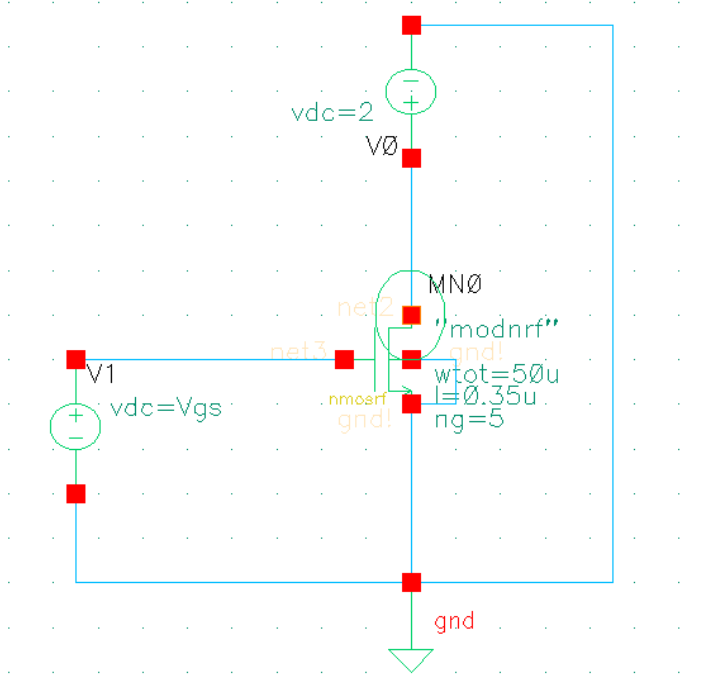
\includegraphics[width=\linewidth]{Q1-schematic.png}
      \label{fig:dctransistor}
  \end{subfigure}%
  \begin{subfigure}[t]{.6\linewidth}
    \centering
    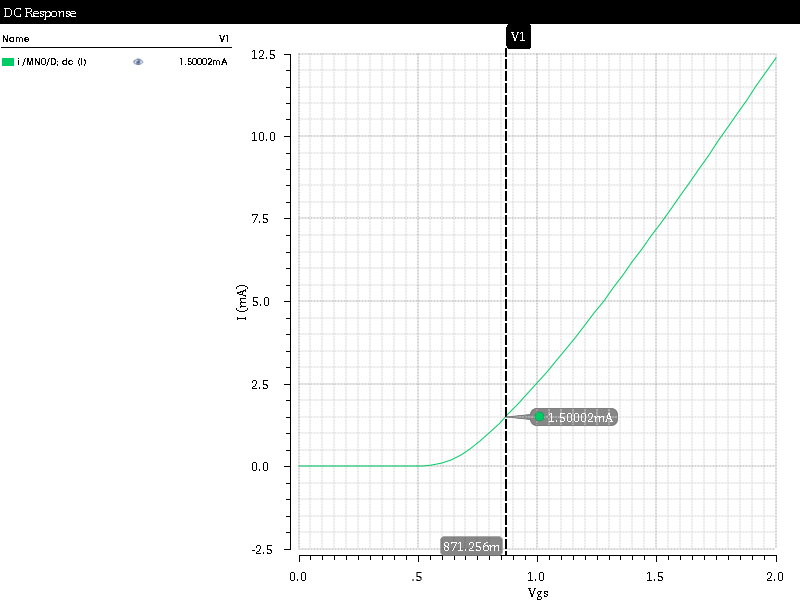
\includegraphics[width=\linewidth]{Q1-IDS_VGS.png}
    \label{fig:dctransistor-sim}
  \end{subfigure}%
  \caption{Sch\'ema et Simulation du circuit $I_{DS} = f(V_{gs})$}
  \label{fig:DCtransistor-simulation}
\end{figure}

On fait une simulation en faisant varier (sweep) le param\`etre $V_{gs}$ afin de trouver $I_{ds0}$ r\'epondant au cahier des charges.
On trouve que pour $I_{DS0} = 1.5 mA$ indiqu\'e dans le cahier de charge, on prend
$V_{gs} = 871.25 mV$.

En effectuant une impression des r\'esultats pour les valeurs de la simulation DC (operating point) :
\begin{itemize} \itemsep -3pt
  \item $V_{gs} = 0.861 V$
  \item $V_t = 0.5563 V$
  \item $V_{OD} = V_{gs} - V_{t} = 0.308V$
  \item $g_m = 7.796 m\Omega$
  \item $I_{ds} = 1.5 mA$
  \item $C_{gs} = 46.37 nF$
\end{itemize}

\clearpage

\subsection{Adaptation de la partie r\'eelle de l'imp\'edance d'entr\'ee}

On r\'ealise le sch\'ema suivant pour v\'erifier l'adaptation en entr\'ee :

\begin{figure}[!htb]
\begin{center}
  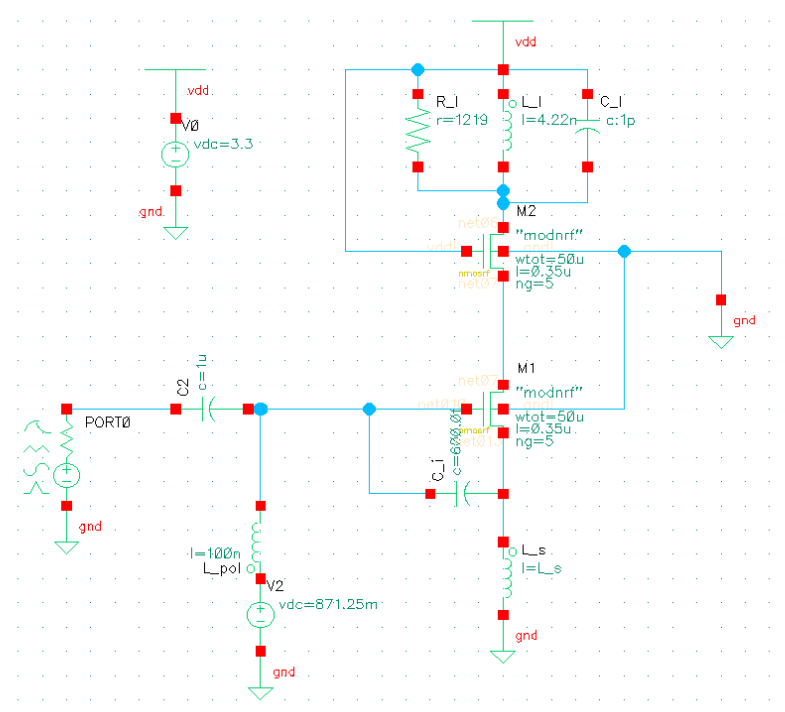
\includegraphics[scale=0.35]{Q2-schematic-adaptation.png}
  \caption{Sch\'ema de l'amplificateur faible bruit pour l'adaptation en entr\'ee}
  \label{lna-adaptation}
\end{center}
\end{figure}

On effectue une simulation SP en entr\'ee en ins\'erant un port, et on cherche \`a trouver les
param\`etres $S_{11}$ en Z-Smith, DB20 et $Re\{Z_{11}\}$.

\begin{figure}[!htb]
\begin{center}
  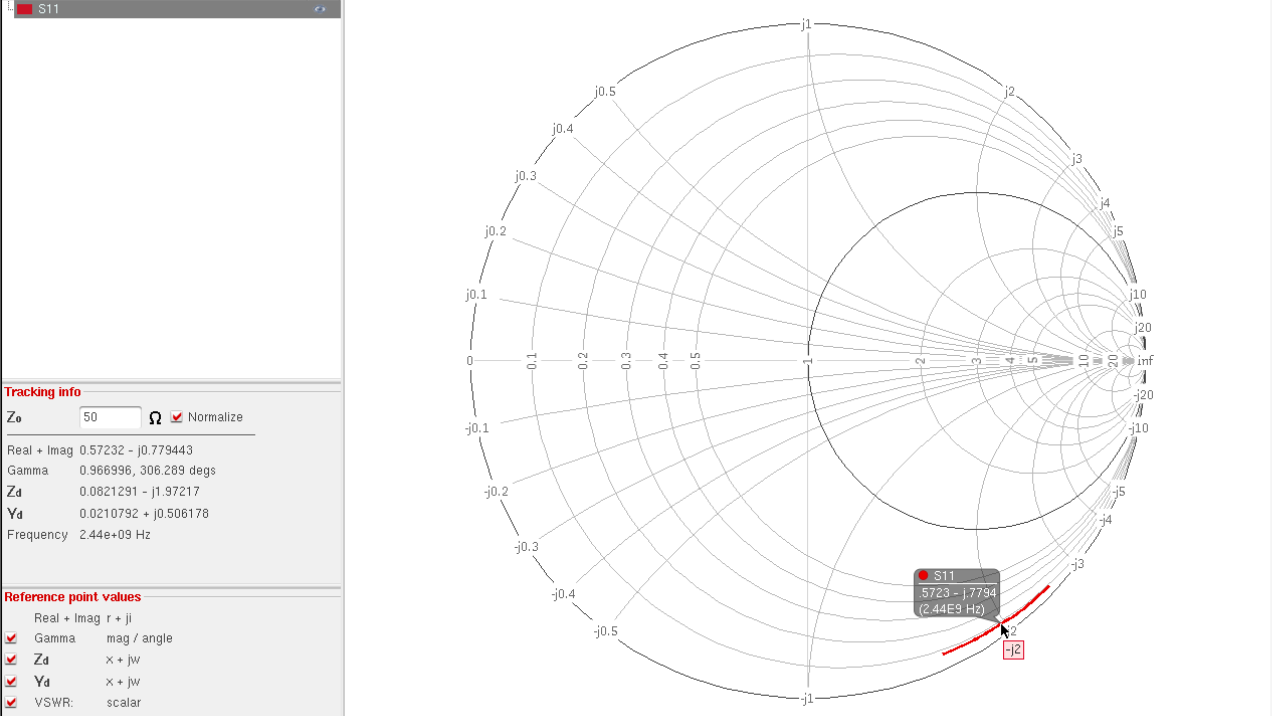
\includegraphics[width=\linewidth]{Q2-S11-Smith-notadapted.png}
  \caption{Abaque de Smith pour $S_{11}$ en entr\'ee }
  \label{S11-nonadapted}
\end{center}
\end{figure}

L'adaptation en entr\'ee n'est pas r\'ealis\'ee, on a $Im\{Zin\}$ non null et $Re\{Zin\}$ diff\'erent de $50 \Omega$.
\clearpage

\begin{figure}[!htb]
  \begin{subfigure}[t]{.5\linewidth}
      \centering
      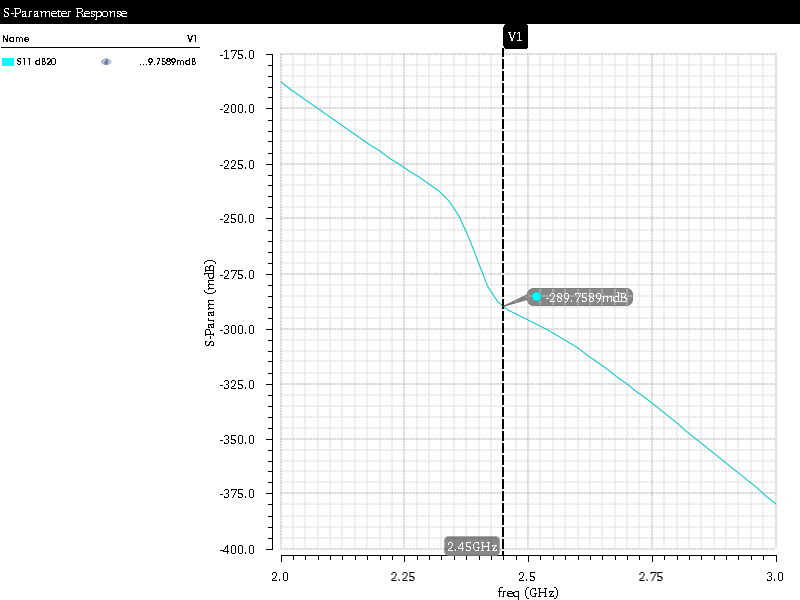
\includegraphics[width=1.1\linewidth]{Q2-dB20-notadapted.png}
      \label{fig:nonadaptedDB20}
  \end{subfigure}%
  \begin{subfigure}[t]{.5\linewidth}
    \centering
    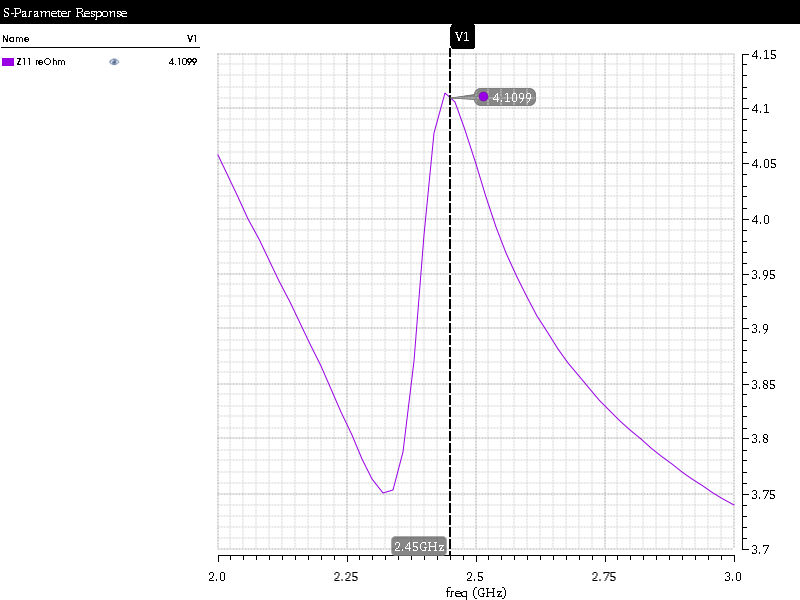
\includegraphics[width=1.1\linewidth]{Q2-realZ11-notadapted.png}
    \label{fig:nonadaptedrealZ11}
  \end{subfigure}%
  \caption{$S_{11}$ en DB20 et $Re\{Z_{11}\}$ respectivement}
  \label{fig:nonadaptedrealZ11-DB20}
\end{figure}

On peut voir qu'il faut modifier la valeur de $L_S$ pour \'etablir la bonne
adaptation. En effectuant une simulation param\'etrique avec $L\_S$ en param\`etre
pour arriver \`a $Re\{Z_{11}\} = 50 \Omega$ en entr\'ee, on a :

\begin{figure}[!htb]
\begin{center}
  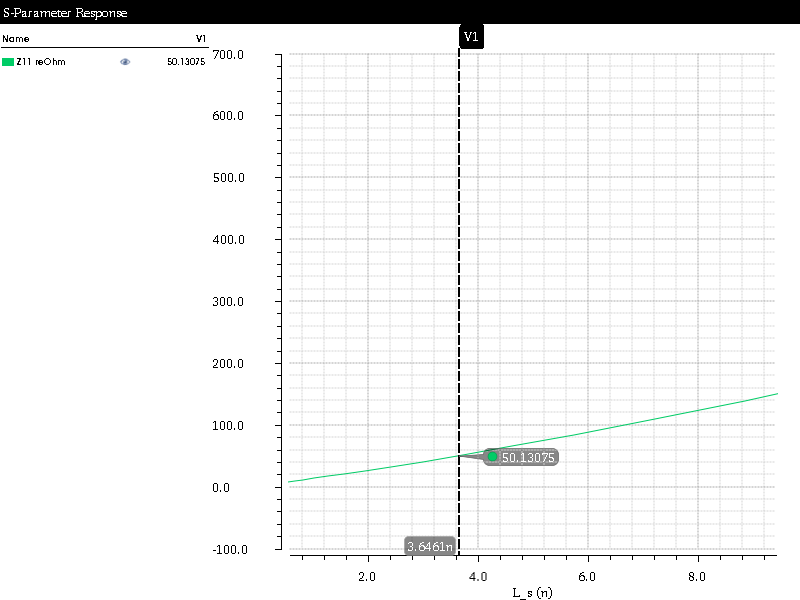
\includegraphics[width=0.7\linewidth]{Q2-C-sim-adaptation.png}
  \caption{Simulation pour arriver \`a $Re\{Z_{11} = 50 \Omega\}$ en entr\'ee }
  \label{RES11-param-LS}
\end{center}
\end{figure}

Ce qui nous donne $L_S = 3.6461 nH$ pour une bonne adaptation.

\clearpage

On reffectue une simulation pour $S_{11}$ en entr\'ee pour Z-smith, DB20 et $Re\{Z_{11}\}$ :

\begin{figure}[!htb]
\begin{center}
  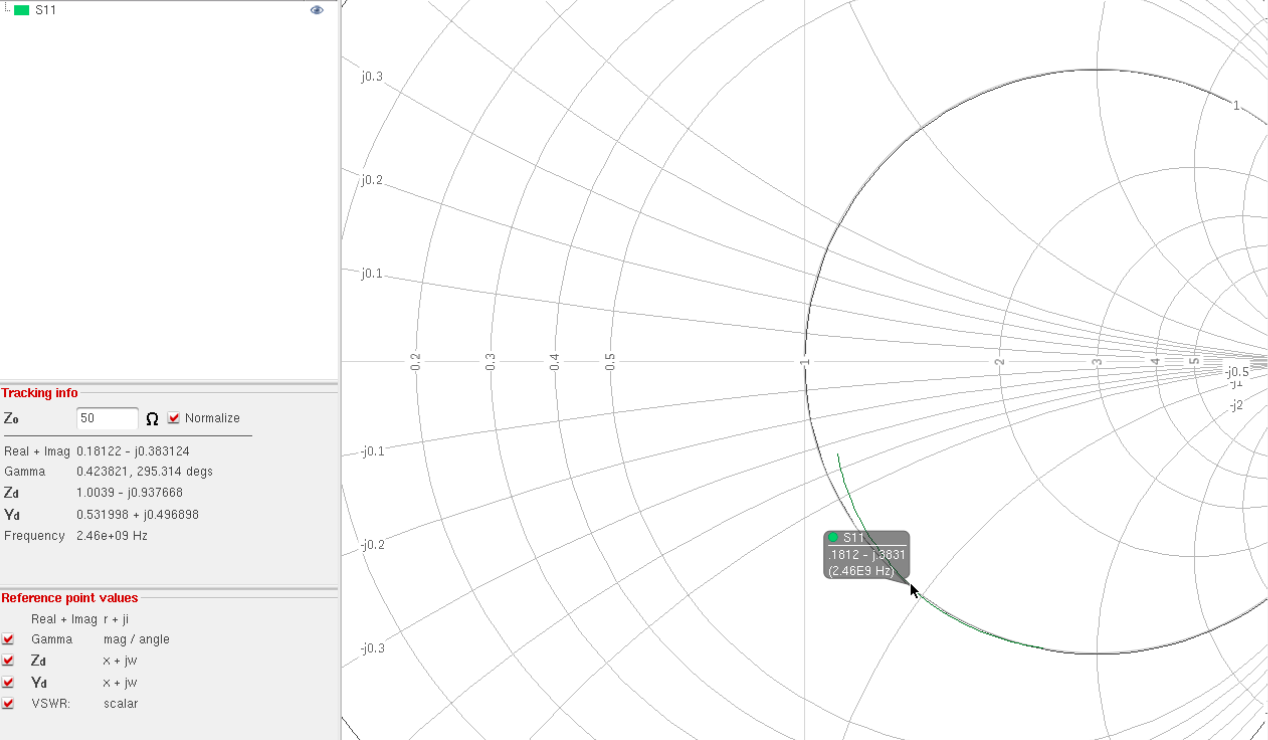
\includegraphics[width=\linewidth]{Q2-S11-Smith-adapted.png}
  \caption{Abaque de Smith pour $S_{11}$ en entr\'ee pour une bonne adaptation }
  \label{S11-adapted}
\end{center}
\end{figure}

\begin{figure}[!htb]
  \begin{subfigure}[t]{.5\linewidth}
      \centering
      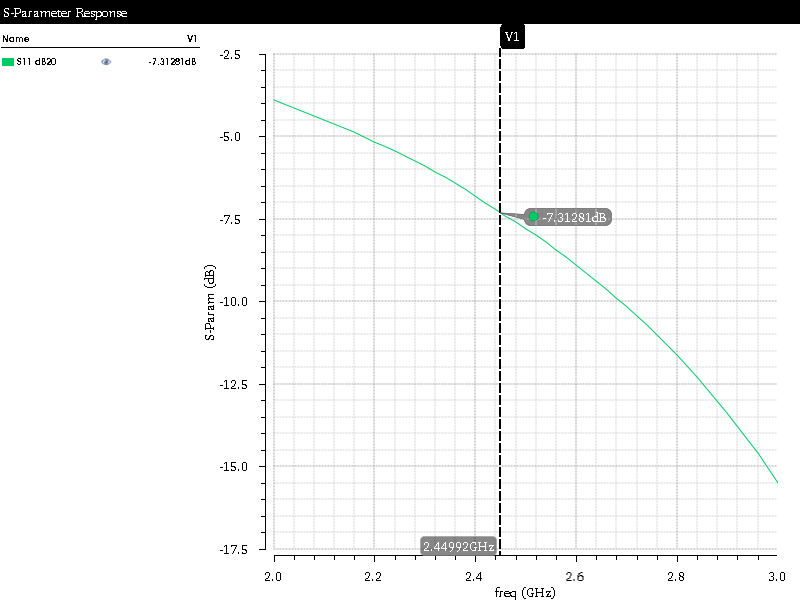
\includegraphics[width=1.1\linewidth]{Q2-dB20-adapted.png}
      \label{fig:adaptedDB20}
  \end{subfigure}%
  \begin{subfigure}[t]{.5\linewidth}
    \centering
    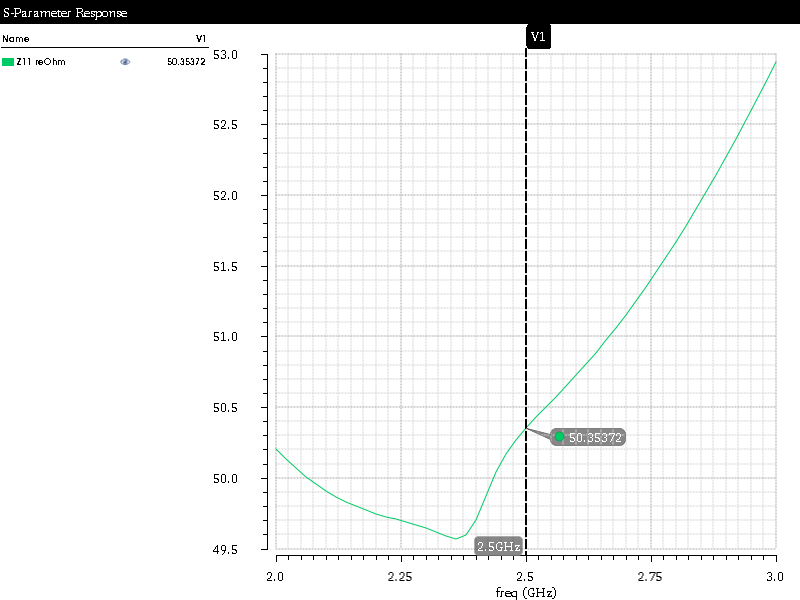
\includegraphics[width=1.1\linewidth]{Q2-realZ11-adapted.png}
    \label{fig:adaptedrealZ11}
  \end{subfigure}%
  \caption{$S_{11}$ en DB20 et $Re\{Z_{11}\}$ respectivement, en \'etablissant l'adaptation en entr\'ee}
  \label{fig:adaptedrealZ11-DB20}
\end{figure}

\clearpage

\subsection{Polarisation}

On ajoute le transistor $M_3$, $R_{pol}$ ainsi que $R_{RF}$ :

\begin{figure}[!htb]
\begin{center}
  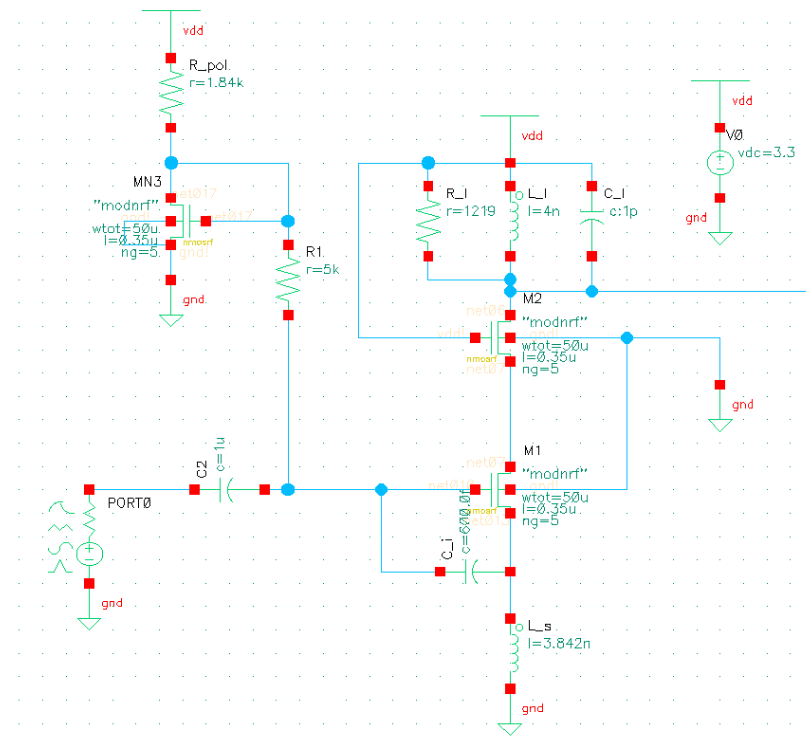
\includegraphics[scale=0.35]{schema-polarization.png}
  \caption{Sch\'ema de l'amplificateur faible bruit avec une polarisation non id\'eale}
  \label{schema-pol}
\end{center}
\end{figure}

Pour garder la m\^eme valeur de $V_{OD} = 0.861V$, on effectue une simulation param\'etrique
pour la valeur de $R_{pol}$, et en regarde la tension \`a l'entr\'ee de $M_{1}$  :

\begin{figure}[!htb]
\begin{center}
  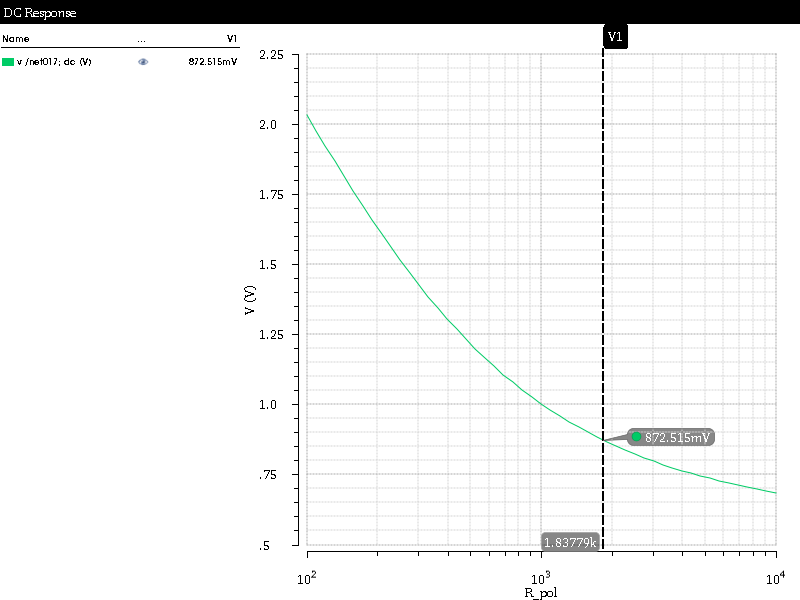
\includegraphics[scale=0.45]{Q3-Rpol-sweep.png}
  \caption{Simulation en prenant $R_{pol}$ en param\`etre}
  \label{schema-pol}
\end{center}
\end{figure}

On retrouve $R_{pol} = 1.833 k\Omega$ pour $V_{OD} = 0.861V$.\\
Note sur $R_{Rf}$ : La r\'esistance remplace une inductance de choke sachant qu'on n'a pas
de courant qui passe au niveau des transistors $M_1$ et $M_3$ donc on peut mettre une r\'esistance
(pas de chute de tension).

\clearpage
L'ajout d'un circuit de polarisation a l'effet de modifier l'adaptation en entr\'ee :
il faut remodifier $L_S$ pour adapter aux changements :

En reffectuant les simulation de $S_{11}$ en entr\'ee, on peut bien v\'erifier l'adaptation
selon les anciennes valeurs : $db_{20}(S_{11}) = -7.5 db$ et $Re\{S_{11}\} = 50 \Omega$.

\begin{figure}[!htb]
\begin{center}
  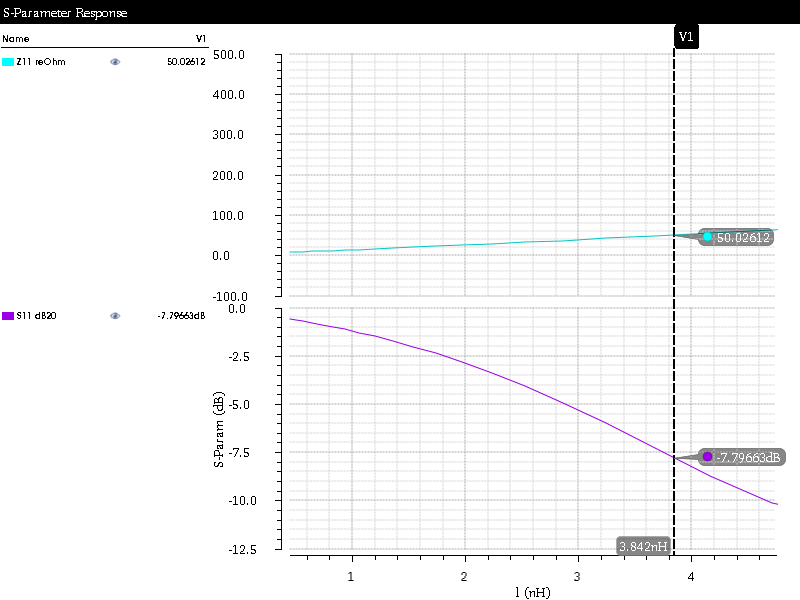
\includegraphics[scale=0.45]{Q3-newLs.png}
  \caption{Valeurs de $S_{11}$ et $Re\{S_{11}\}$ pour une simulation en prenant $L_S$ en param\`etre}
  \label{newLS}
\end{center}
\end{figure}

On retrouve une nouvelle valeur de $L_S$ : $L_S = 3.842 nH$.

\vskip 3 cm

\subsection{Gain}
En effectue une simulation SP selon 2 ports, pour s'en faire, on ajoute un port \`a la sortie du LNA:

\begin{figure}[!htb]
\begin{center}
  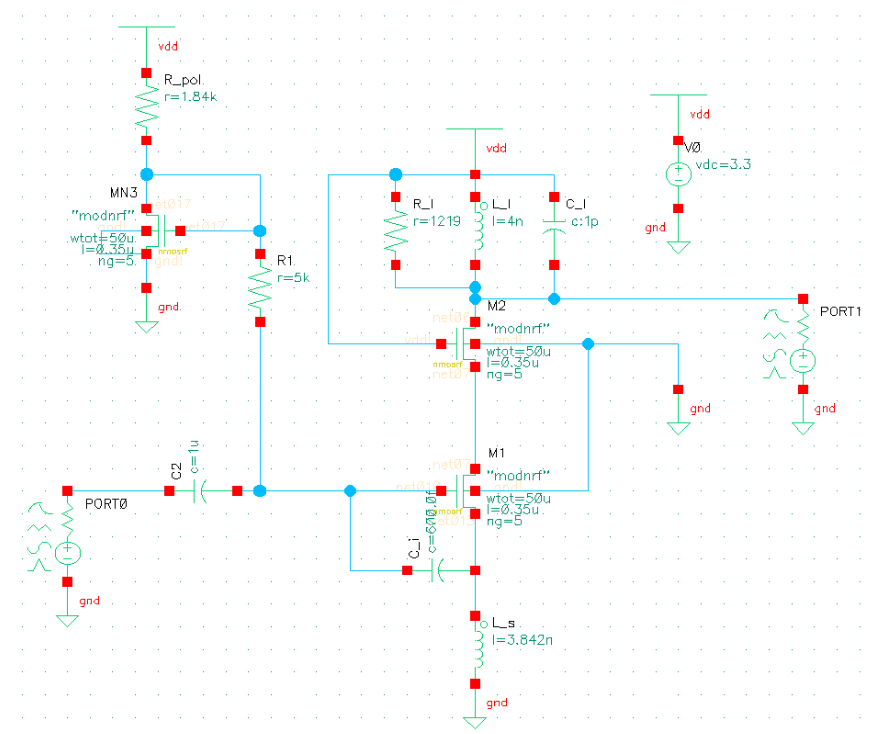
\includegraphics[scale=0.30]{schematic_lna_global.png}
  \caption{Sch\'ema de l'amplificateur faible bruit complet avec un port en sortie}
  \label{schema-pol}
\end{center}
\end{figure}

\clearpage

On effectue une simulation en cherchant $S_{21}$ :

\begin{figure}[!htb]
\begin{center}
  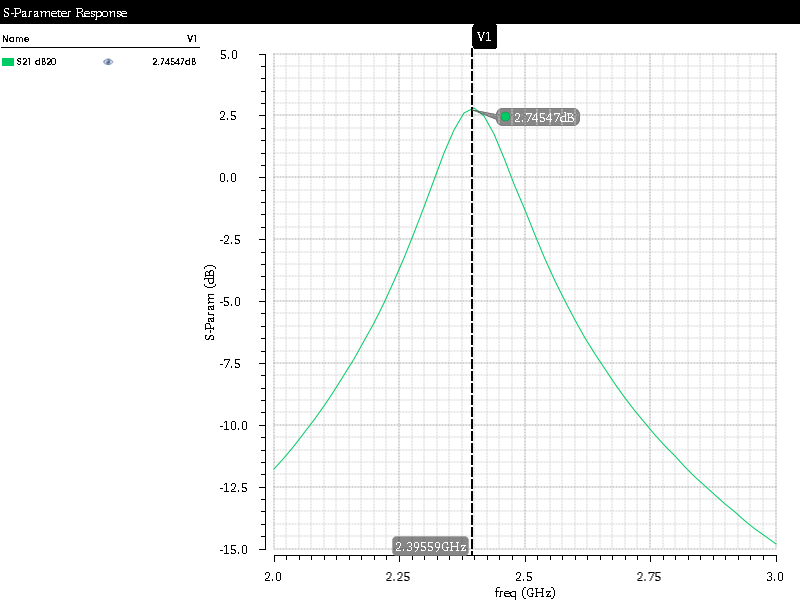
\includegraphics[scale=0.45]{Q4-S21.png}
  \caption{Simulation SP de $db_{20} (S_{21})$ en sortie du LNA}
  \label{schema-pol}
\end{center}
\end{figure}

On voit qu'il y a un d\'ecalage en fr\'equence. Celui-ci est due \`a la valeur de $L_L$.

On cherche $L_L$ pour obtenir une adaptation maximale, en effectuant un sweep sur ses valeurs.

\begin{figure}[!htb]
\begin{center}
  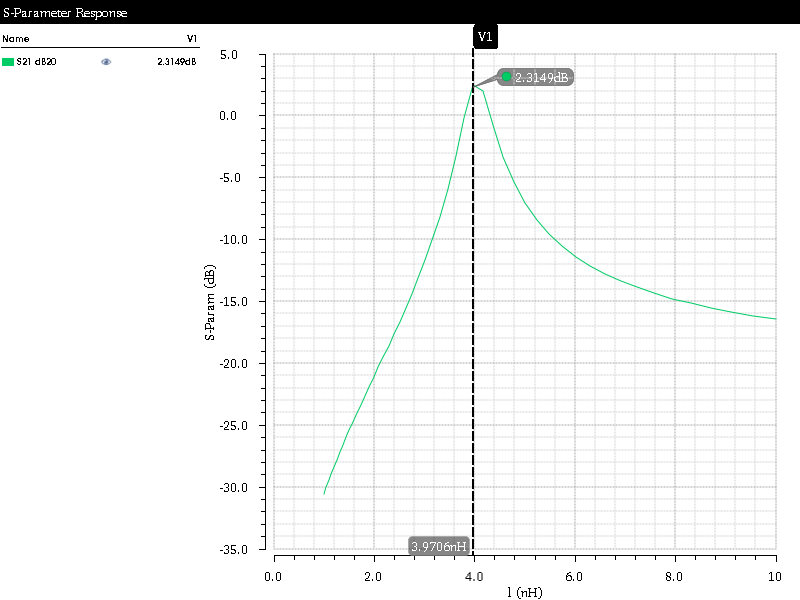
\includegraphics[scale=0.45]{Q4-S21-newL_l.png}
  \caption{Simulation SP de $db_{20} (S_{21})$ en fonction d'une variation $L_L$ }
  \label{newLL}
\end{center}
\end{figure}

\clearpage

Avec cette valeur de $L_L = 3.9706 nH$, on arrive \`a retrouver le $S_{21}$ max :

\begin{figure}[!htb]
\begin{center}
  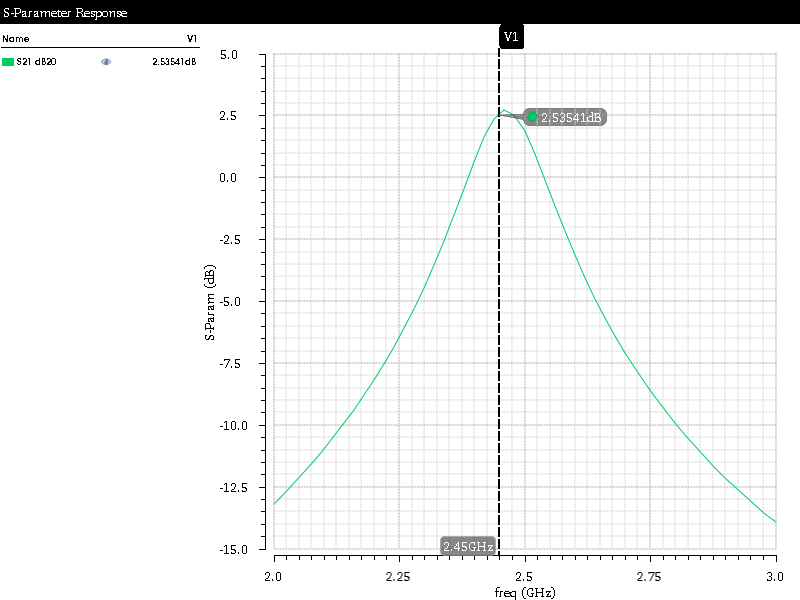
\includegraphics[scale=0.45]{Q4-S21db20-newL_l.png}
  \caption{Simulation SP de $db_{20} (S_{21})$ pour une bonne valeur de $L_L$}
  \label{s21-sp-sim-newll}
\end{center}
\end{figure}

\textbf{Calcul de la valeur de $G_v$(dB)}

On a :
\[
  S_{21} = \frac{
    \sqrt{
      \frac{V^2_{out}}{R_{out}}
    }
  }
  {
    \sqrt{
    \frac{V^2_{in}}{R_{in}}
    }
  }
  = \frac{V_{out}}{V_{in}} \frac{\sqrt{\frac{1}{R_{out}}}}{ \sqrt{\frac{1}{R_{in}} } } = \frac{V_{out}}{V_{in}} \sqrt{\frac{R_{in}}{R_{out}} }
\]
\[
\implies 20log(S_{21}) = 20 log(G_v) + 20 log \bigg( \bigg(\frac{R_{in}}{R_{out}}\bigg)^{0.5}\bigg)
\]
d'ou
\[
G_v\big|_{db} = S_{21}\big|_{db} - 10 log \bigg(\frac{R_{in}}{R_{out}}\bigg)
\]
ou m\^eme :
\[
G_v\big|_{db} = S_{21}\big|_{db} + 10 log \bigg(\frac{R_{out}}{R_{in}}\bigg)
\]
On arrive \`a obtenir : $G_v\big|_{db} = 22.5 dB \implies$ On a une diff\'erence de $26 - 22.5 = 3.45 db$


\begin{figure}[!htb]
\begin{center}
  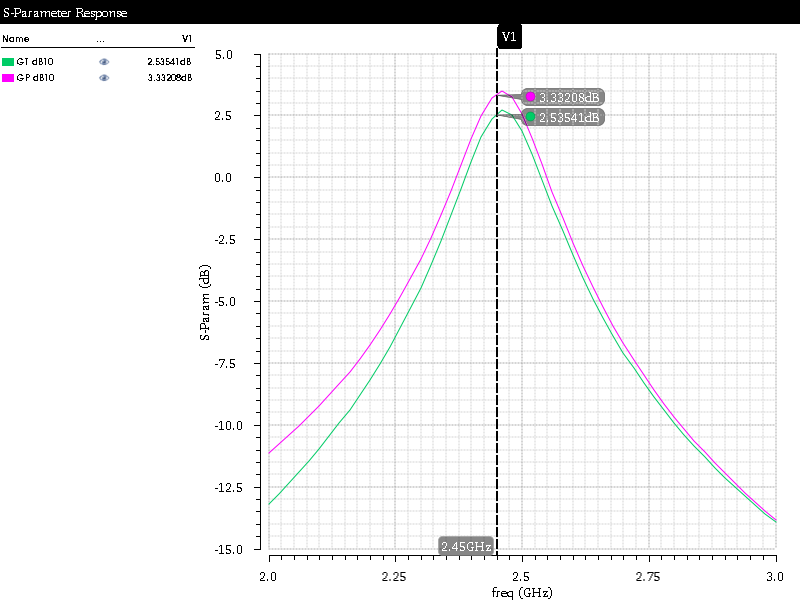
\includegraphics[scale=0.45]{Q4-GT-GP-db20.png}
  \caption{Simulation SP de $db_{20}$ ($G_T$) et ($G_P$) }
  \label{sim-GT-GP}
\end{center}
\end{figure}

\clearpage

On peut retrouver les expressions de $G_T$ et $G_P$ :
\begin{equation*}
Gp\ =\ \frac{P_{L}}{P_{in}} \ =\ \frac{|S_{21} |^{2}\left( 1-|\Gamma _{L} |^{2}\right)}{( 1-S_{22} \Gamma _{L})^{2}\left( 1-|\Gamma _{in} |^{2}\right)}
\end{equation*}
et :

\begin{equation*}
  G_{T} \ =\ \frac{P_{L}}{P_{av}} \ =\ \frac{|S_{21} |^{2}\left( 1-|\Gamma _{L} |^{2}\right)\left( 1-|\Gamma _{S} |^{2}\right)}{|1-\Gamma _{in} \Gamma _{S} |^{2} |1-S_{22} \Gamma _{L} |^{2}}
\end{equation*}

Quand on est bien adapt\'e en entr\'ee et en sortie, on retrouve $G_T = G_P$.

\begin{figure}[!htb]
\begin{center}
  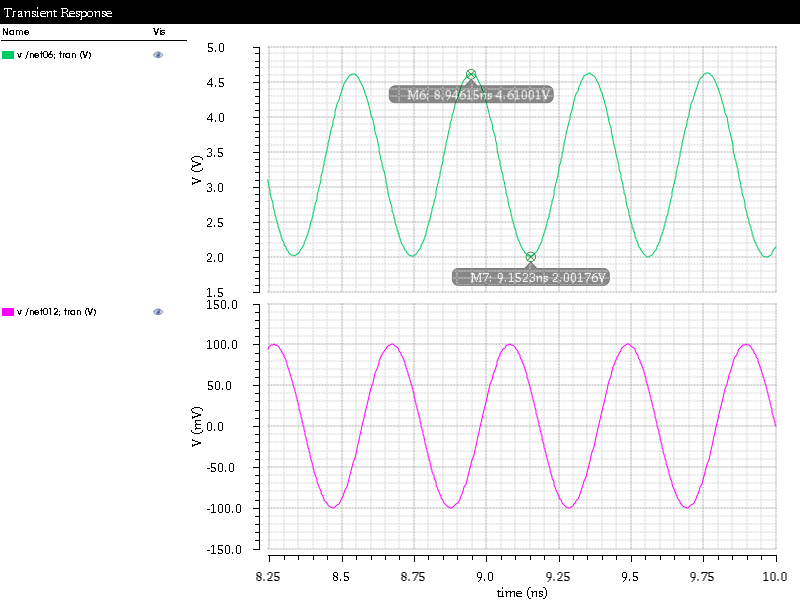
\includegraphics[scale=0.45]{Q4-Gv-tran.png}
  \caption{V\'erification du gain en par une simulation transiant}
  \label{sim-transiant-gv}
\end{center}
\end{figure}

Pour la simulation transitoire, on met une tension d'entr\'ee $V_{in} = 0.1 V$ de fr\'equence $f = 2.45 GHz$.\\
On a selon fig. \ref{sim-transiant-gv} , $Vout = 1.3 V$.
Ce qui implique que :
\[
G_V = \frac{V_{out}}{V_{in}} = \frac{1.3}{0.1} = 13
\]
d'ou $G_V = 20log(13) = 22.5 dB$.

\subsection{Adaptation de la partie imaginaire de l'imp\'edance d'entr\'ee du LNA}
On ajoute $L_i$ et on effectue un sweep pour $f=2.45GHz$ en fonction de la valeur de $L_i$
pour obtenir une valeur o\`u $G_T = G_P$ :

\begin{figure}[!htb]
\begin{center}
  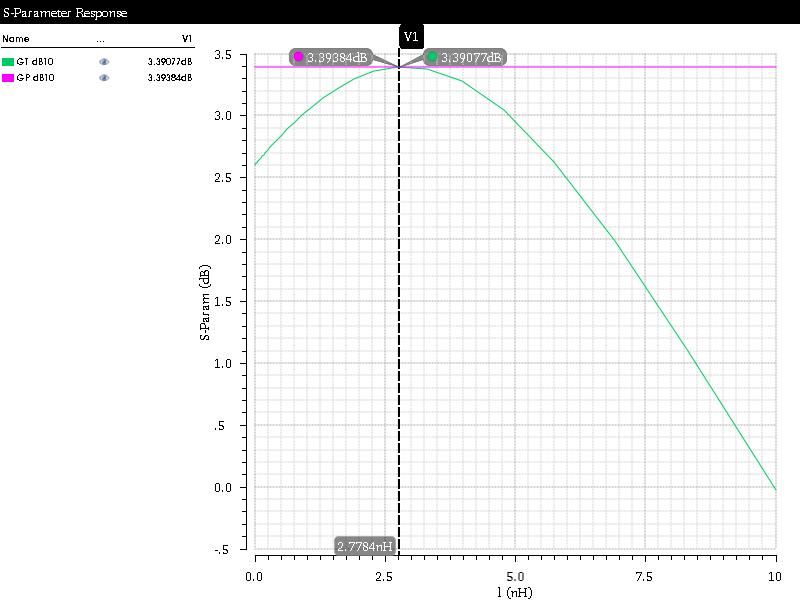
\includegraphics[scale=0.35]{Q5-L_i-sweep.png}
  \caption{Sweep des valeurs de $L_i$ pour arriver \`a $G_T = G_P$}
  \label{sim-li-sweep}
\end{center}
\end{figure}

On retrouve $L_i = 2.7784 nH$.\\

\clearpage

On v\'erifie ce r\'esultat en fonction de la fr\'equence :

\begin{figure}[!htb]
\begin{center}
  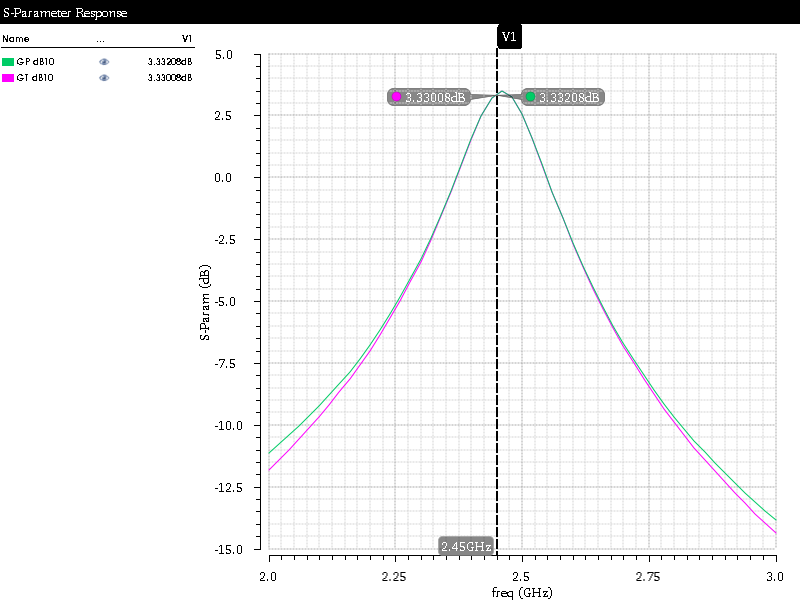
\includegraphics[scale=0.45]{Q5-GT-GP-db20.png}
  \caption{Simulation SP de $G_T$ et $G_P$  }
  \label{sim-li-gt-gp}
\end{center}
\end{figure}

On v\'erifie aussi la bonne adaptation (pour $S_{11}$) :


\begin{figure}[!htb]
\begin{center}
  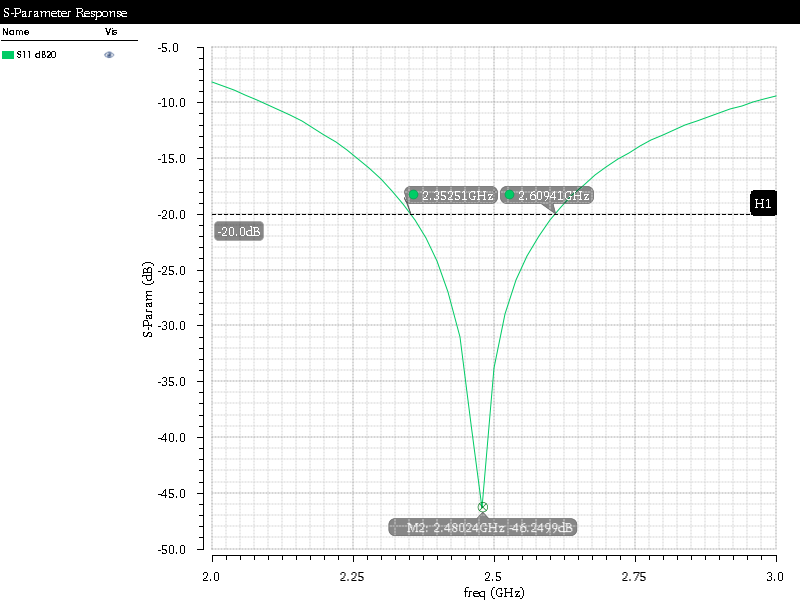
\includegraphics[scale=0.45]{Q5-S11-db20.png}
  \caption{Simulation SP de $G_T$ et $G_P$  }
  \label{sim-q5}
\end{center}
\end{figure}

Fonction de $L_i$ : Li sert \`a adapter l'entr\'ee en annulant la partie imaginaire de Zin.\\
Par rapport au $S_{11}$ :  Si on est parfaitement adapt\'e \`a $50 \Omega$  pour $f= 2.45GHz$, $S_{11}$ tends vers
$-\infty$, il n'y a aucun retour d'onde, toute la puissance est transmise.

\clearpage
\subsection{Facteur de bruit}

Facteur du bruit :

\begin{figure}[!htb]
\begin{center}
  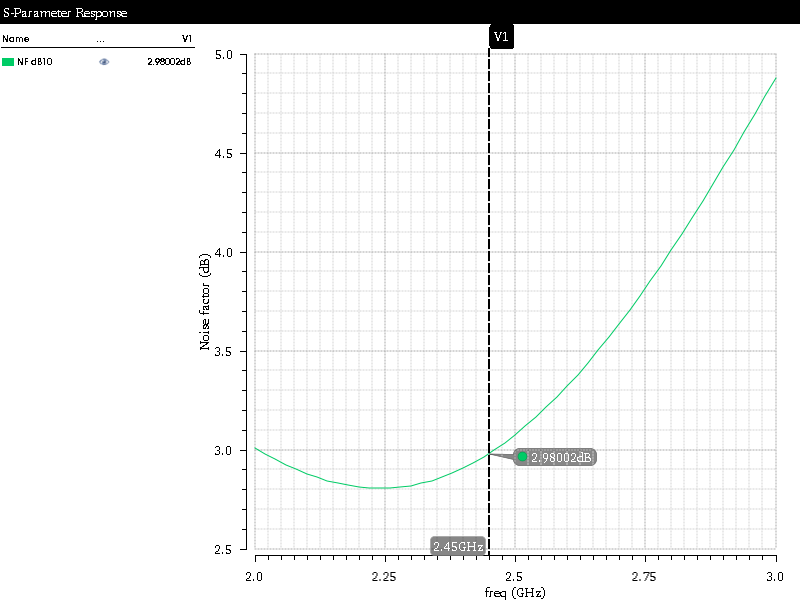
\includegraphics[scale=0.45]{Q6-NF-dB10.png}
  \caption{Simulation en $db_{10}$ du Noise factor}
  \label{facteur-bruit}
\end{center}
\end{figure}

On retrouve que le facteur de bruit c'est $NF= 2.98 dB$ pour $f=2.45GHz$.



Point de compression \`a 1 db :

\begin{figure}[!htb]
\begin{center}
  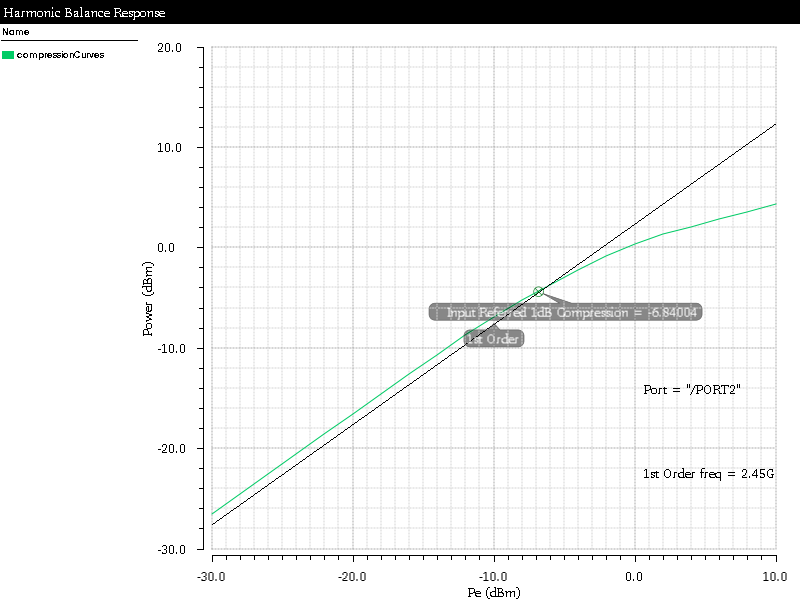
\includegraphics[scale=0.45]{Q6-1dB_Compression.png}
  \caption{Simulation en $db_{10}$ du point de compression 1db}
  \label{facteur-bruit}
\end{center}
\end{figure}

On trouve qu'il faut redimensioner le transistor $M_{1}$ pour arriver \`a un NF r\'eduit :
 $\implies$ On augmente le W \`a 150 $\mu m$.

il faut refaire une adaptation en entr\'ee pour  1.76 dB (Sachant qu'on a augment\'e le W).
Pour $W = 150 \mu m$, on retrouve $I_{DS0} = 4.519 mA$
Sachant que :
\[
  I_{DS} = \frac{1}{2}{C_{ox}}{\mu_n} \frac{W}{L}(V_{GS} - V_{Th})^2
\]
$\implies$ Si $W' = 3W \implies$ $I'_{DS0} = 3I_{DS0} = 3 \times 1.5 mA$

\clearpage

\begin{figure}[!htb]
\begin{center}
  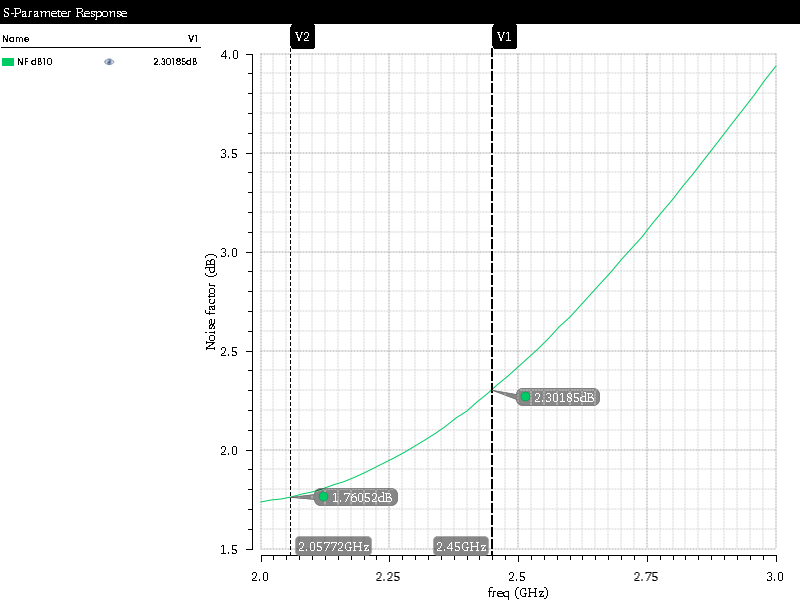
\includegraphics[scale=0.40]{Q6-NF-dB10-bigW.png}
  \caption{Simulation du NF : On arrive \`a un NF r\'eduit pour une fr\'equence plus basse}
  \label{facteur-bruit}
\end{center}
\end{figure}

On effectue une simulation DC operating point pour retrouver la valeur de $I_{DS}$.
On retrouve bien une valeur de $I_{DS}$ anticip\'ee.

\begin{figure}[!htb]
\begin{center}
  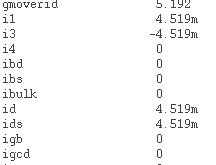
\includegraphics[scale=0.40]{Q6c-Ids0.png}
  \caption{Simulation DC}
  \label{facteur-bruit}
\end{center}
\end{figure}

On refait une simulation SP pour v\'erifier le $NF = 1.76dB$  ainsi que les gains GT et GP
pour $f=2.45 GHz$. On retrouve qu'on est plus adapt\'e en entr\'ee
pour une valeur diff\'erente de W : il faut refaire l'adaptation, en r\'eglant $L_i$,$L_S$.\\
On passe \`a $L_i = 6.02 nH$ pour annuler la partie imaginaire de l'imp\'edance en entr\'ee,
$L_s = 1.68 nH$, pour arriver \`a un $Re\{Z_e\}=50$. \\
On arrive a une bonne adaptation ainsi qu'un Gain $>$ 6db, mais on est d\'ecaler en fr\'equence,
on fait une adaptation de $L_L$, en effectuant un sweep de $L_L$ pour retrouver un max de $G_T$
$\implies L_L = 3.8 nH$.


\begin{figure}[!htb]
\begin{center}
  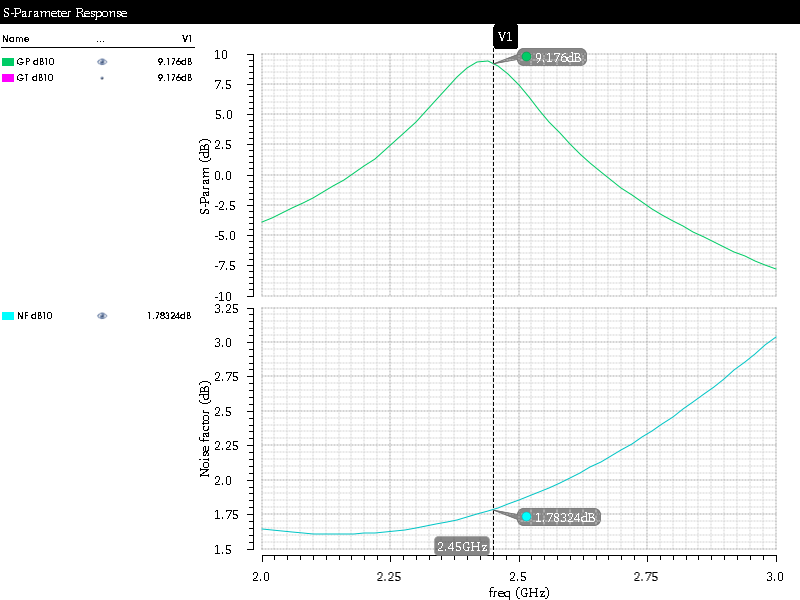
\includegraphics[scale=0.45]{Q6c-GTGP-NFdB10.png}
  \caption{Simulation }
  \label{facteur-bruit}
\end{center}
\end{figure}


\clearpage
\section*{Conclusion}
\addcontentsline{toc}{section}{Conclusion}


Ce TP de conception d'un LNA nous a permis de reprendre quelques \'el\'ements d'adaptation vus en TP1 tout en approfondissant l'\'etude avec
 des simulations plus avanc\'ees (harmonic balance, simulations de bruit) afin de d\'eterminer le gain, le point de compression et le NF.
 Nous avons \'egalement pu observer les gains GT et GP afin de d\'eterminer l'adaptation en entr\'ee.
 
Pour la partie diff\'erentielle, nous avons polaris\'e les transistors mais nous n'avons pas pu simuler correctement tout le montage.


\addcontentsline{toc}{section}{R\'ef\'erences}
\begin{thebibliography}{9}

\bibitem{RFIC-tp-lna}
\textit{Conception d'un LNA \`a 2.45 GHz en Technologie 0.35 $\mu$m AMS - \'Enonc\'e de TP}\\
\texttt{Institut Polytechnique de Grenoble - Phelma}

\bibitem{RFIC-cours}
\textit{Radio Frequency Integrated Circuits Course}\\
\texttt{Sylvain Bourdel, Florence Podevin, Institut Polytechnique de Grenoble - Phelma}

\bibitem{conception-adaptation}
\textit{Conception d'un circuit en L \`a l'aide de l'abaque de Smith}\\
\texttt{http://f5zv.pagesperso-orange.fr/RADIO/RM/RM23/RM23p/RM23p03.html}

\bibitem{Analog-CMOS-microelectronics}
\textit{Design of Analog CMOS Integrated Circuits, 2nd Edition}\\
\texttt{Behzad Razavi, McGraw-Hill Education}

\bibitem{conception-circuits-integrees}
\textit{Conception de circuits int\'egr\'es analogique}\\
\texttt{Laurent Aubard, Institut Polytechnique de Grenoble - Phelma}

\end{thebibliography}


\end{document}
